\section{吸收作用与微聚焦}
\label{sec:3.1}

有时,地层因不规则性很小而呈水平产状,在这种情况下,我们也许有希望不采用偏
移。地震射线应适合于大炮检距上出现大反射角时的简单模型,这样的资料对于观测作为
角度之函数的反射系数、或者对于观测地层的地震能量吸收率$1/Q$,都是很理想的资料。Ei-
nar Kjartansson在其博士论文中就曾报导过这类研究,其结论颇富启发性,所以本节 将详
细评论一下该项研究。我不知道Grand Isle气田在何种程度上可以典型代表其他的地层, (Pan, 1983
),但要想了解关于炮检距的意义,这儿对初学者却是个好地方。

\subsection{Grand Isle气田:典型的亮点}
\label{sec:3.1.1}

Kjartansson所研究的是一条通过路易斯安娜(Louisiana)州海岸外的Grand
Isle气田的地震测线资料,该项资料系由海湾石油公司提供。该项资料在某种相当平缓的原产层面
上,含有若干典型的“亮点”(强反射)。具有意义的是:在约为2.3秒的时间深度上的反
射中,出现了振幅的横向变化(见以下的图\ref{fig:ofs/kjcos}),普遍相信这类亮点是由浅层含气砂岩
形成的。

理论预言,反射系数应是角度的函数。对于像气饱和砂岩这样的一种异常物理情况,该种
函数理应具有与众不同的特点,在如图\ref{fig:ofs/kjcos}所示的共中心点道集
中将可发现其存在的证据。观察这些道集中的任何一个道集时,
你都会注意到反射强度对炮检距
的关系似乎是一种平滑的、表现灵敏的函数,从外表上看完全杲
可测定的。可是,利用层状介质理论已能确定,只有最不可能的异
乎寻常的介质才能表现出反射系
数随角度而有如此强的变化,尤其是在很小的入射角时(时间2.5秒时达到很宽炮检距时的反
射角并不是一个很大角度,若假设速度为常数,则该角度为28°,
即$arccos(2.3/2.6)=28°$)。使人困惑不解的是,各个共中心点道集都表现为某种不同的光滑
和反应灵敏的可观测函数。此外,这些中心点彼此靠近,十个炮
点所张之水平距离不过才820英尺。
\begin{figure}[H]
\centering
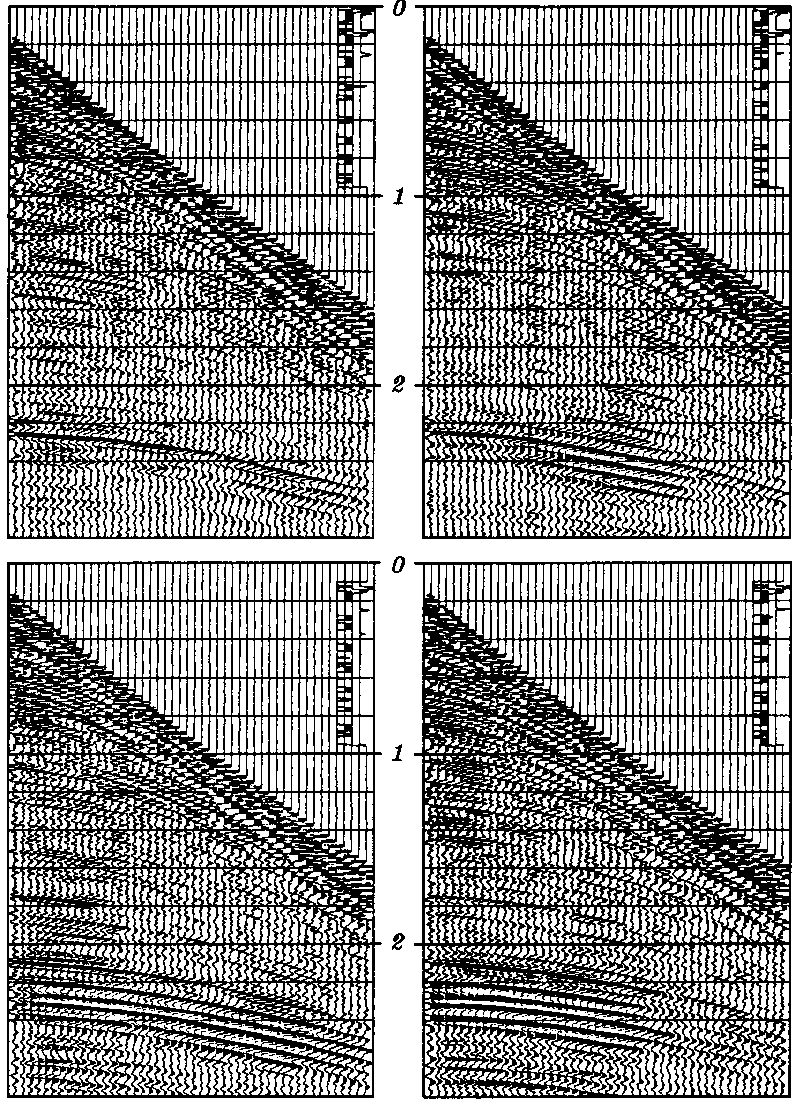
\includegraphics[width=0.65\textwidth]{ofs/kjcmg}
\caption[kjcmg]{顶部左侧为炮点220;右侧为炮点230。除与时间成比例的显示增益之外,未
进行任何处理。底部所示为炮点305与315(Kjartansson,海湾石油公司)}
\label{fig:ofs/kjcmg}
\end{figure}

\subsection{Kjartansson的振幅横向变化模型}
\label{sec:3.1.2}

根据以层状介质理论为基础的模型来看,Grand
Isle的资料是难以理解的,于是Kja-
rtansson提出了另一种不同的模型。图\ref{fig:ofs/kjidea}所示即是这种模型,
其中,呈直线形式的射线由任何震源入射至平缓水平反射面,然后再反射至接收点。其复杂化仅在于介质中存在有一
些“透镜状”的物体,它们以某种异常的方式干扰了地震射线。开始时你也许会猜想这些透
镜体吸收了地震波能量(干扰结杲到底是由能量聚焦所形成还是由能量吸收所形
成,最终述是搞不清楚)。

透镜体A接近于地表,地震勘探结果 两次受它影响——一次是当炮点横向通过
该透镜体时,一次是当检波器横向通过该透镜体时。透镜体C位于反射面附近并包
含它的一小部分面积,在所有炮检距$h$上
均可见该透镜体,怛仅见其位于中心点$y_0$。图\ref{fig:ofs/kjidea}顶部图形所示射线路程是一
种受到所有透镜体影晌的路程,透镜体位于中心点且从最远炮检距心$h_{max}$处可见;
从图\ref{fig:ofs/kjidea}底部图形中可知其射线路程。
\begin{figure}[H]
\centering
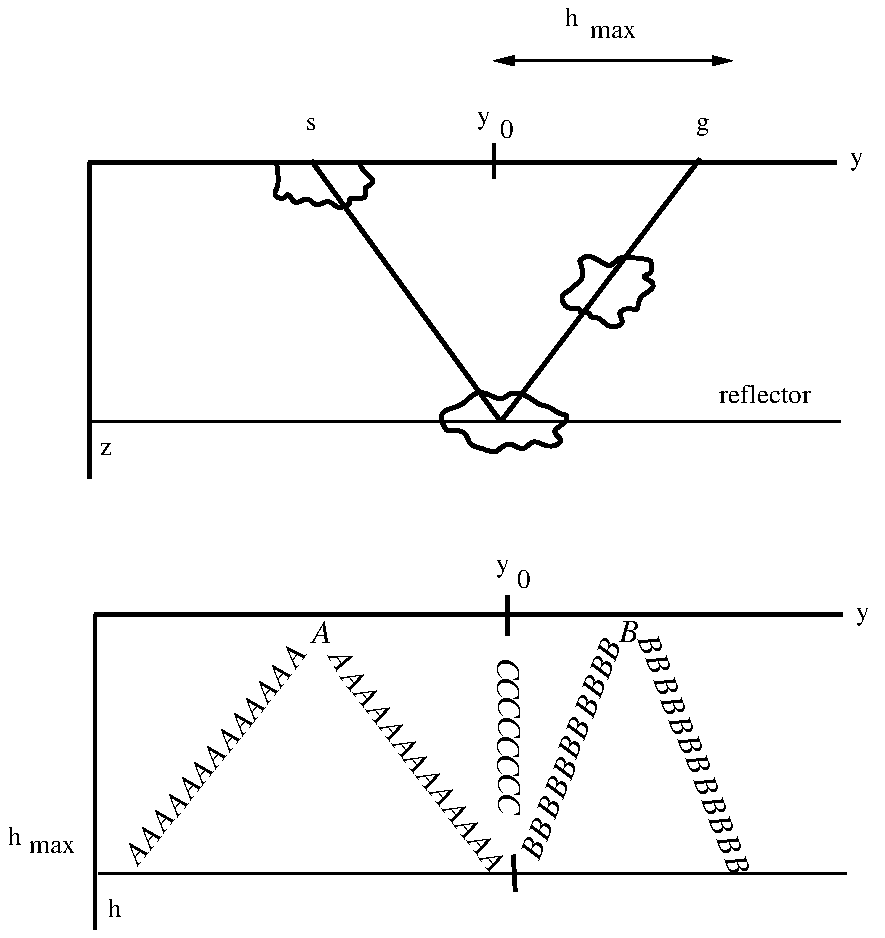
\includegraphics[width=0.65\textwidth]{ofs/kjidea}
\caption[kjidea]{Kjartansson模型。上图为模型,下图为该模型所产生的干扰数据
空间示意图。透镜体A、B与C的异常物质可由来自深层的反射所受影响而监测出来。
}
\label{fig:ofs/kjidea}
\end{figure}
图\ref{fig:ofs/kjcos}所示是通过该气田的一个共炮检距剖面,所用
炮检距是近炮间距道一侧的第五记录道,距炮点为1070英尺。别上当受骗
以为水层很深,在大约为0.33秒处的初至其实是广角反射。

在从1.5秒至3秒的时间间隔内计算出各个地震记录的功率,将功率取对数然后作为中心
点与炮检距之函数绘出,如图\ref{fig:ofs/kja}(a)所示。注意,能量条纹大约是
以45°角度横切过$(y,h)$平面,最强的条纹是以准确的45°角度横过170号炮点的近
炮检距道,由图\ref{fig:ofs/kjcos}清楚可
见,这是因为这里丢失了一个炮点。其次,考虑一下可甩模型中的透镜体C来描述的含气砂
岩。观测资料中的任何含气砂岩影响都应当在含气砂岩所在中心点上以横切过所有炮检距的
条纹形式表现出来-一也就是说,该条纹应垂直于坐标$y$。但是,在图\ref{fig:ofs/kja}(a)
中,看不出有这神条纹存在。仔细研究该图即可知,其余许多清晰可见的条纹在该平面上均呈显著小于
±45°的角度。关于图中条纹的角度唯一可能的解释就是:它们很像是透镜体B所形成,这
些透镜体均介于地面与反射面之间。由该角度可以确定其深度,越接近45°角而非接近于
0°角,该透镜体就越接近于地表面而不接近于反射面。

\begin{figure}[H]
\centering
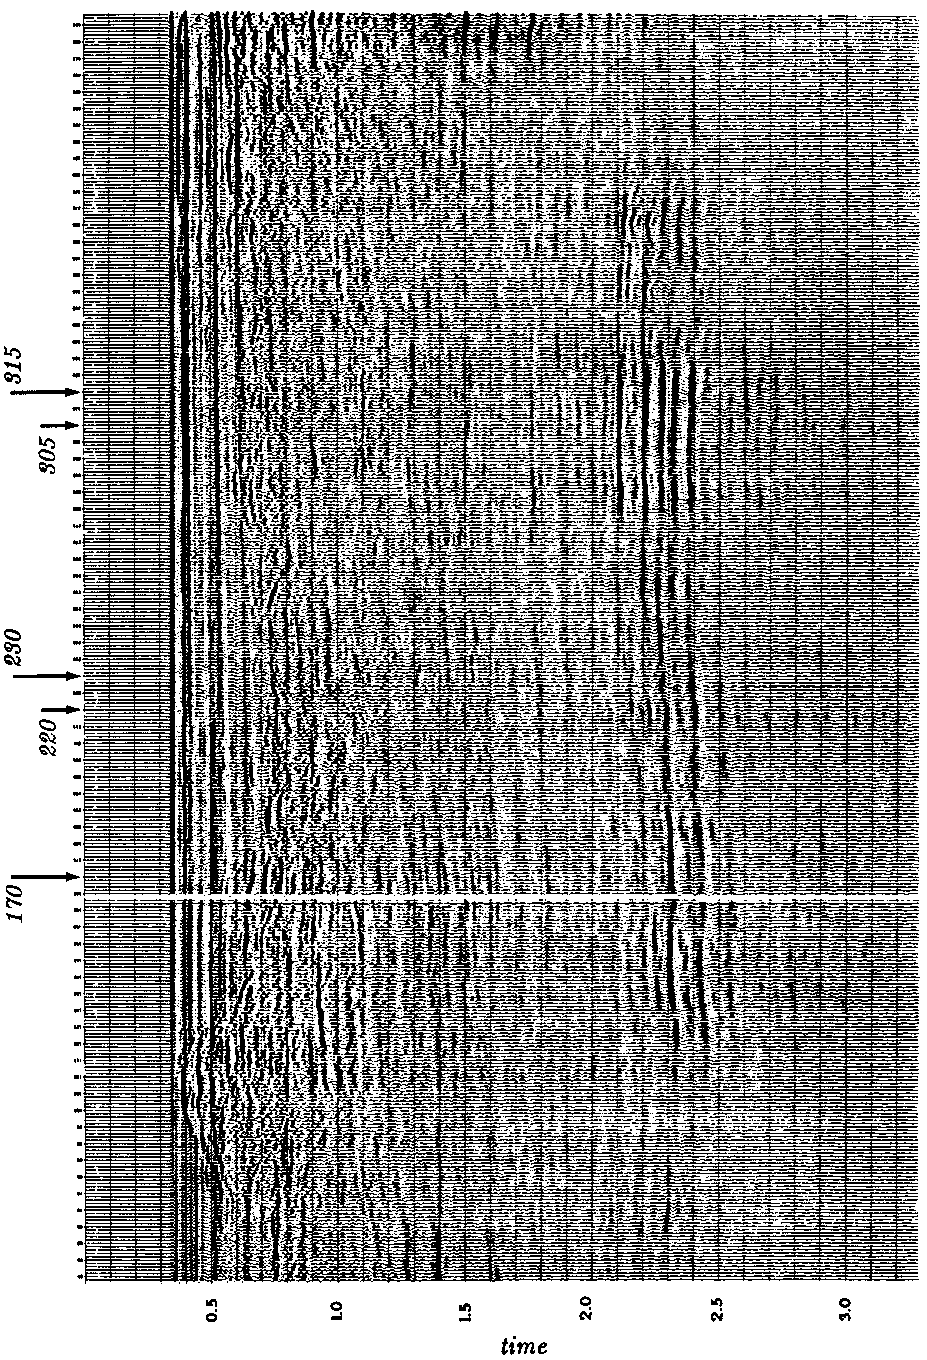
\includegraphics[width=0.65\textwidth]{ofs/kjcos}
\caption[kjcos]{通过Grand Isle气田的一个共炮检距剖面。
所用炮检距属于近记录道的第五记录道(Kjartansson,海湾石油
公司。}
\label{fig:ofs/kjcos}
\end{figure}

\begin{figure}[H]
\centering
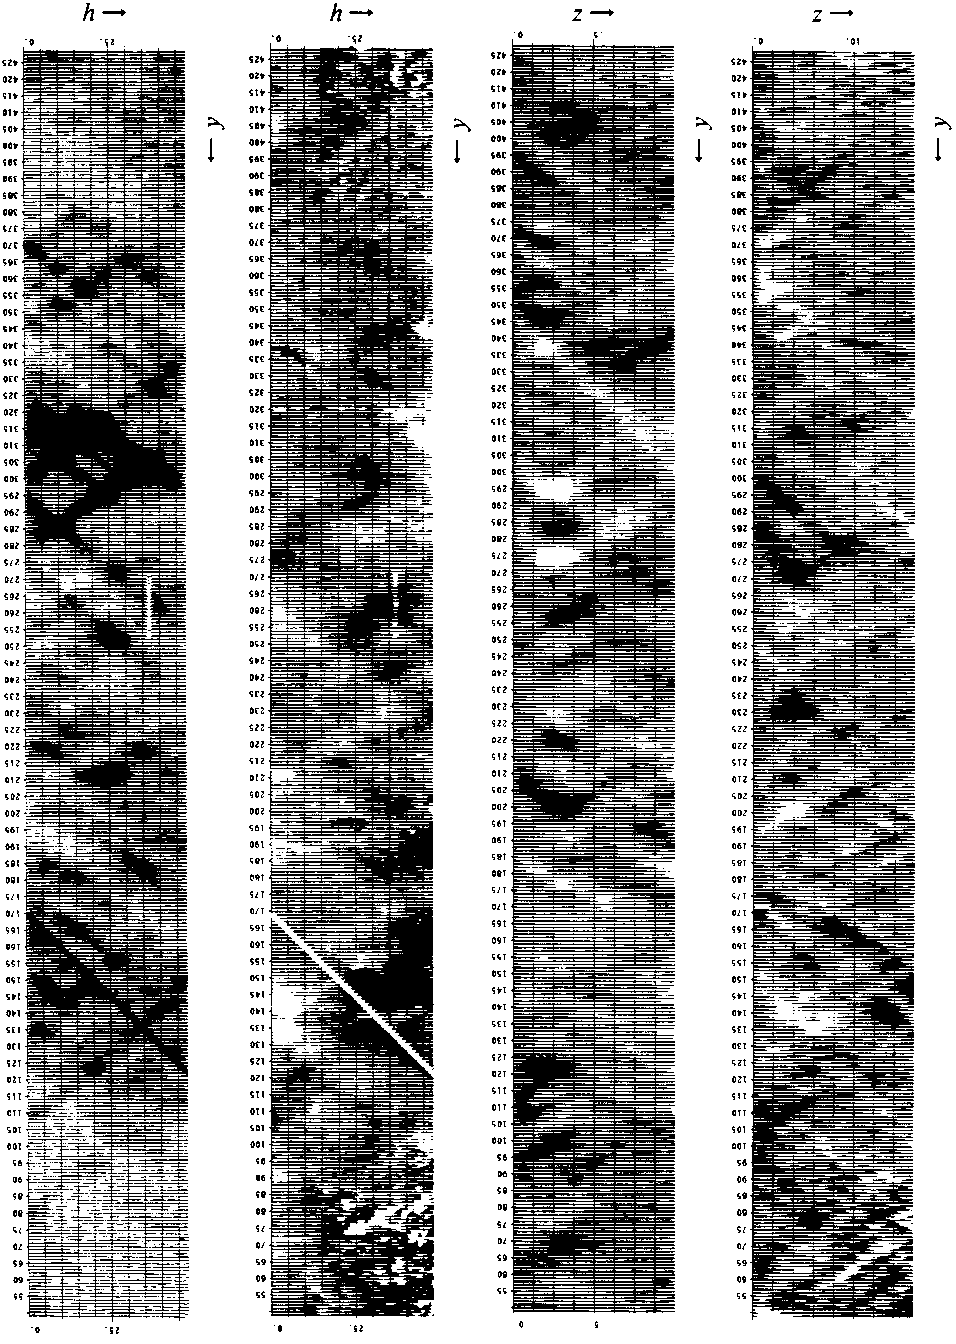
\includegraphics[width=0.65\textwidth]{ofs/kja}
\caption[kja]{从左往右依次是:a)幅度$(h,y)$,b)时间$(h,y)$,
c)幅度$(z,y)$,d)时间$(z,y)$}
\label{fig:ofs/kja}
\end{figure}

以图\ref{fig:ofs/kja}(a)表示幅度的相同方式,在图\ref{fig:ofs/kja}(b)中表示出计时信息。计算出一个共
中心点叠加结杲,然后将每个野外地震记录与其比较,从而确定每个记录道的剩余时差,并
将它们绘于图\ref{fig:ofs/kja}(b)内,图\ref{fig:ofs/kjmid}所示是共中心点道集之一经过动校正之后的情形,其上
的剩余时差清楚可见。

\begin{figure}[H]
\centering
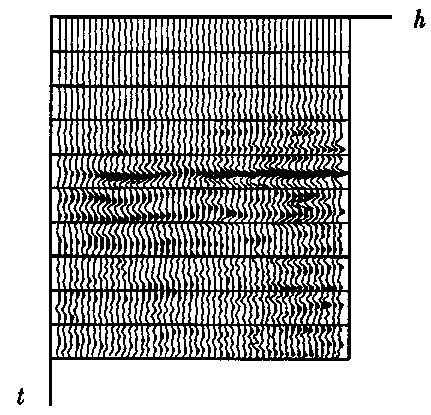
\includegraphics[width=0.65\textwidth]{ofs/kjmid}
\caption[kjmid]{时差校正之后的中心点道集220(与图\ref{fig:ofs/kjcmg}(b)相同)。
所示是中心位于2.3秒处之一秒宽时窗内的情形,根据2.3秒处的同相轴进行时差
校正,所用速度为7000英尺/秒(Kjartansson)}
\label{fig:ofs/kjmid}
\end{figure}

除了幅度较低时出现干扰或者“相位跳跃”使观测发生混乱的地方出现干扰之外,所得
结杲同幅度的情形颇类似。图\ref{fig:ofs/kja}
(b)清楚表明,对时间记时的扰动影响出现在幅度受到扰动时的相同深度上。

在5.2节内阐述的逆倾斜叠加能够使我们决定透镜体的深度分布,这种分布显示于图
\ref{fig:ofs/kja}(c)和\ref{fig:ofs/kja}(d)内。

密西西比河所携带的沉积物沉降在三角洲上,那里有沙坝、边滩、现已淤塞的古河
曲、鸟足状分布砂质支流河道,在各河道之间多沼泽的洪积平原为腐败有机物所充填。这种
自然景观显然是横向可变的,在生长断层和后来沉积物的重量影响下,它最终将全部因其自
身的重量而沉降下去。在它被掩埋而消失不见之后,横向可变性将继续通过透镜体表现出来
而为未来的地震学家们所观测到。这些地震学家也许会看到一神有点像图\ref{fig:ofs/meander}所示那样的
情形。图\ref{fig:ofs/meander}显示的是三维地震勘探结果,就是说,勘探船沿着线距为70米左右的许多平
行测线进行了许多航次的勘探。该图顶面平面是恒定时刻时的一个切片,所示是掩埋了的河
曲,资料的提供者Dahrn与Graebner(1982)比较详尽地描述了图\ref{fig:ofs/meander}所示的资料。
\begin{figure}[H]
\centering
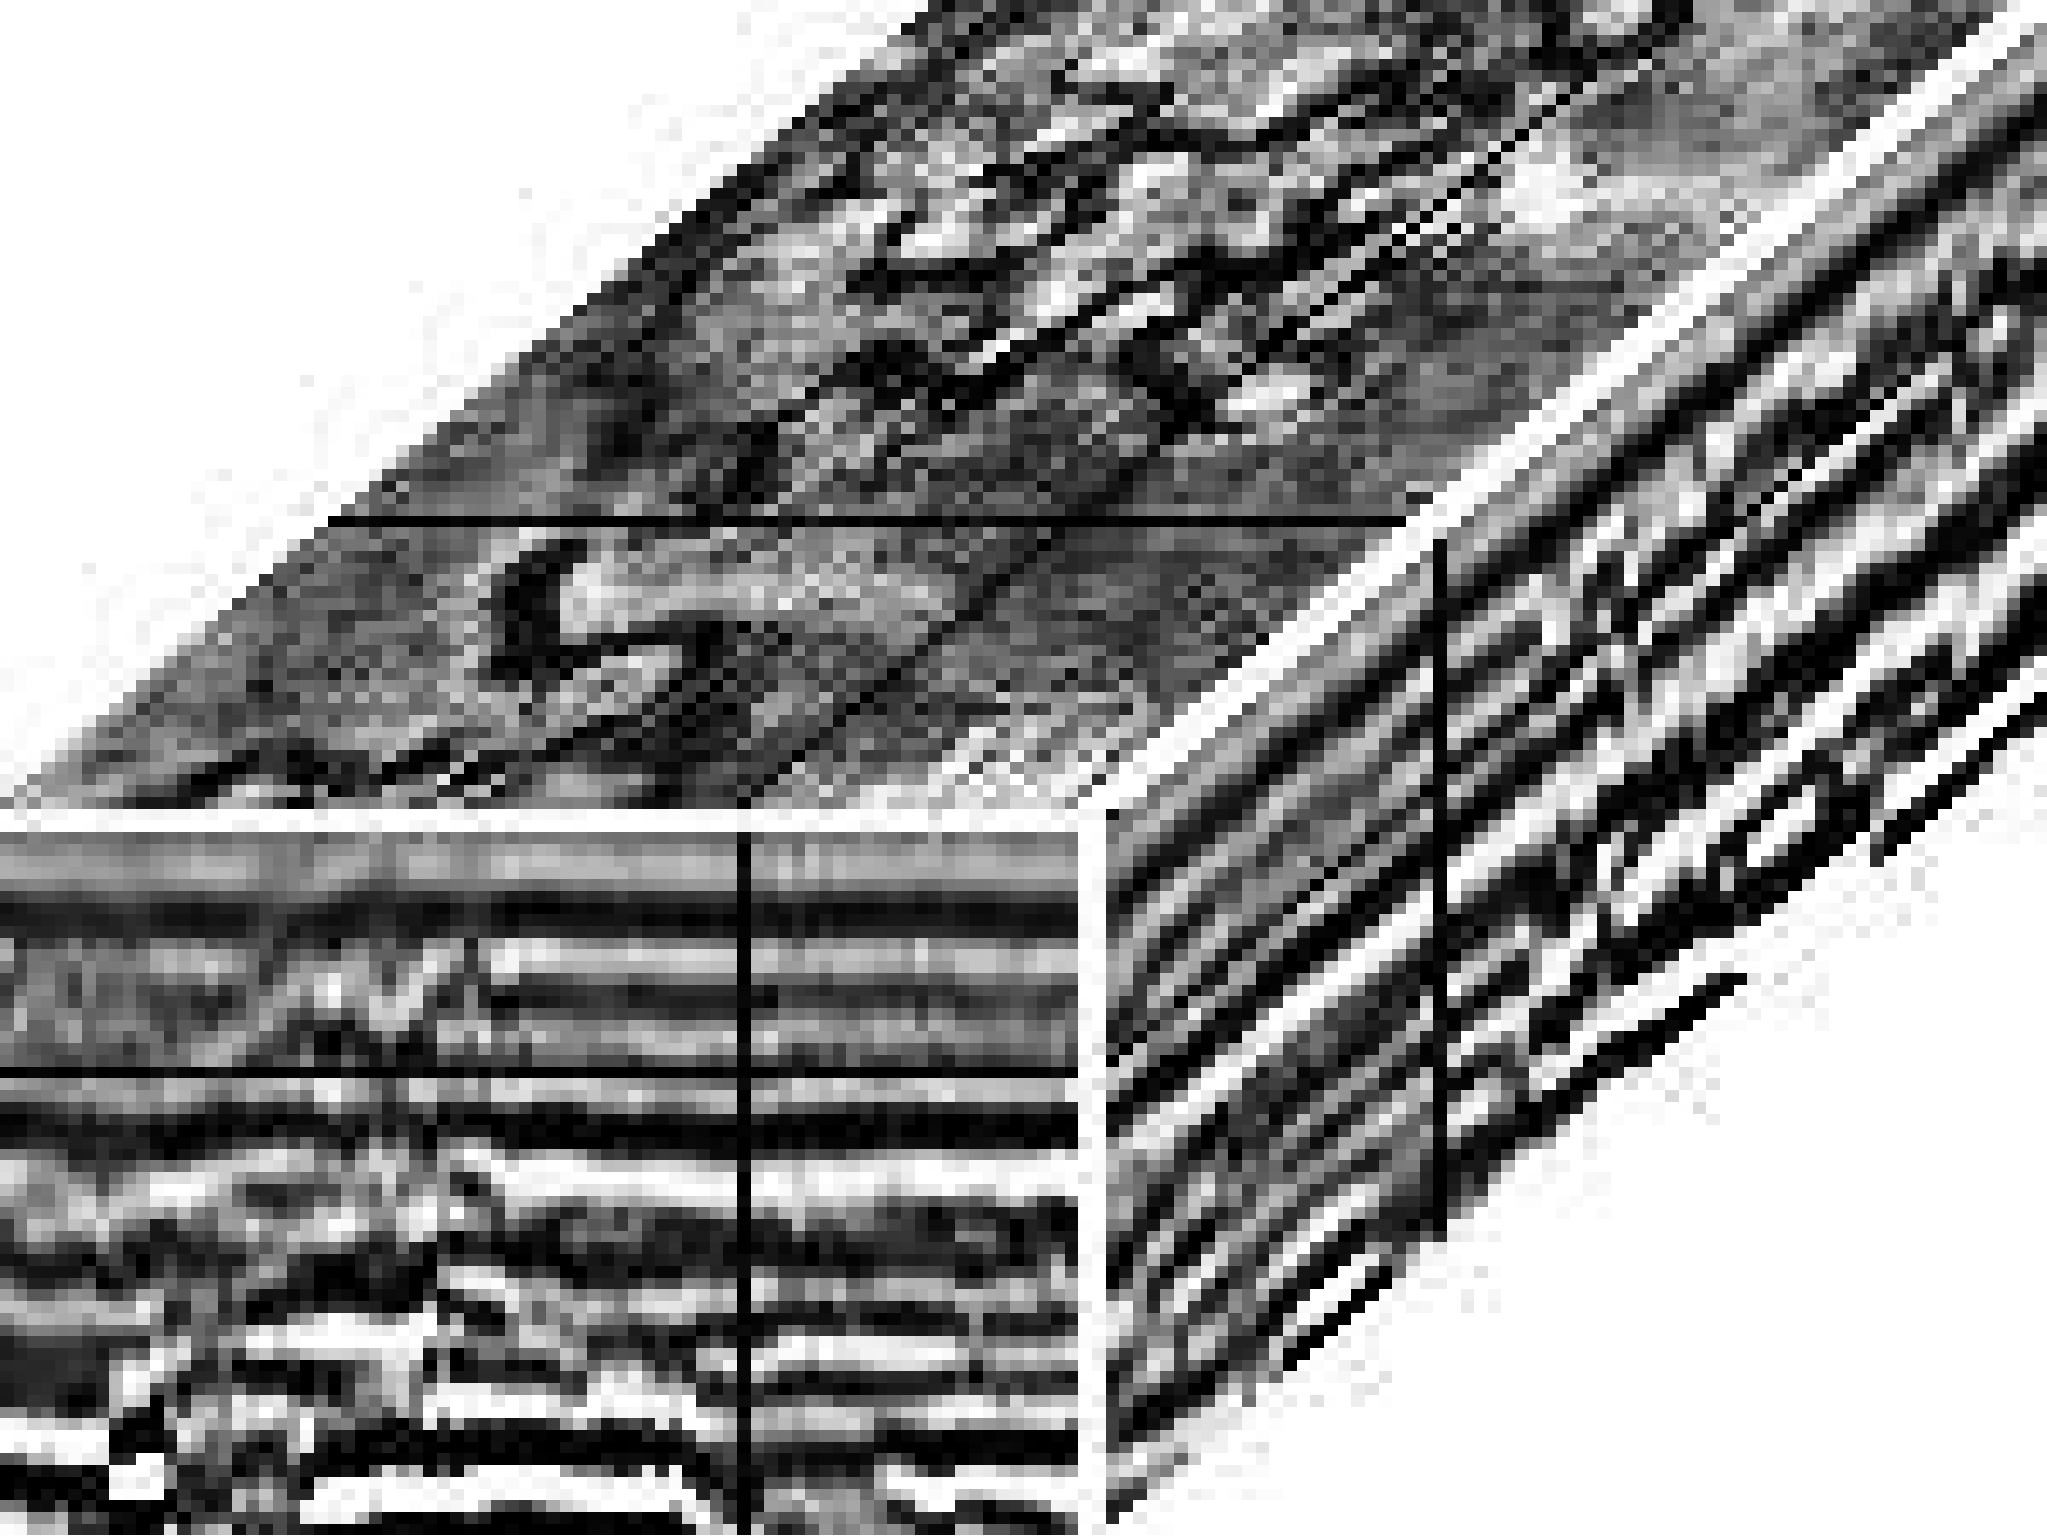
\includegraphics[width=0.65\textwidth]{ofs/meander}
\caption[meander]{泰国海湾地区三维地震资料(Geophysical Services公司)。
立方体内部各数据平面均显示于该立方体的各侧面上,顶部平面表示现已被淹没的古蛇曲河流}
\label{fig:ofs/meander}
\end{figure}

\subsection{聚焦还是吸收?}
\label{sec:3.1.3}

具有高度能量吸收作用的岩石通常都具有低速度。通过一个低速透镜体,按理波动应为吸
收所减弱,但是它们也会因聚焦而加强。究竟哪一种影响占主导地位?这种现象与空间波长有
何关系?完整地恢复一种物理模型,还有许多工作要完成。知道图\ref{fig:ofs/kja}(c)
上的黑色斑点代表低振幅或高吸收,而图\ref{fig:ofs/kja}(d)上的黑色斑点代表低速度,
那末也许你就能够解决这个问题。

\subparagraph{习题}
\label{sec:3.1.4}

\begin{enumerate}
\item   试考虑压力P波转换为剪切S波,设S波速度约为P波速度的二分之一。对于这些
  S波,图\ref{fig:ofs/kjidea}将呈何种形状?
\end{enumerate}
